\section{Arduino kode}
Den indledende løsning blev først implementeret på en arduino uno hvor konceptet blev testet og verificeret.

\begin{figure}[h!]
  \centering
  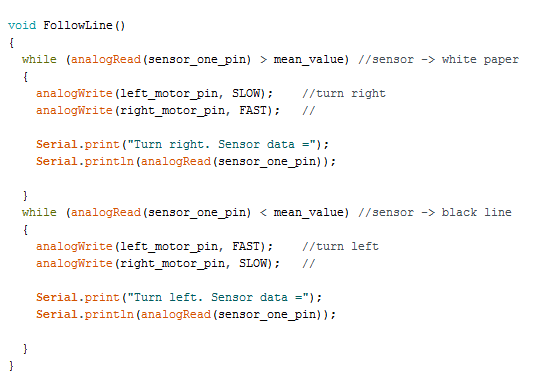
\includegraphics[width=0.6\textwidth]{figures/followLine2.png}
  \caption{FollowLine() funtion.}
  \label{follow_line_kode}
\end{figure}

Koden fungere helt simpelt ved at når sensoren ser den hvide linje drejes der til højre, og når den sorte linje ses, drejes der til venstre. Derved kører roboten kun på kanten af linjen.

\subsection{Test med en sensor}
Ud fra det introducerde linetrack system, testet even til at følge en bane med en sort streg.
